\chapter{Impulsformung}
Leistungsdichtespektrum bei bipolarer Signalisierung mit rechteckfürmigen
Impulsen $p_{rect}(t)$ mit Rate $r_b=\frac{1}{T_b}$:

\begin{center}
	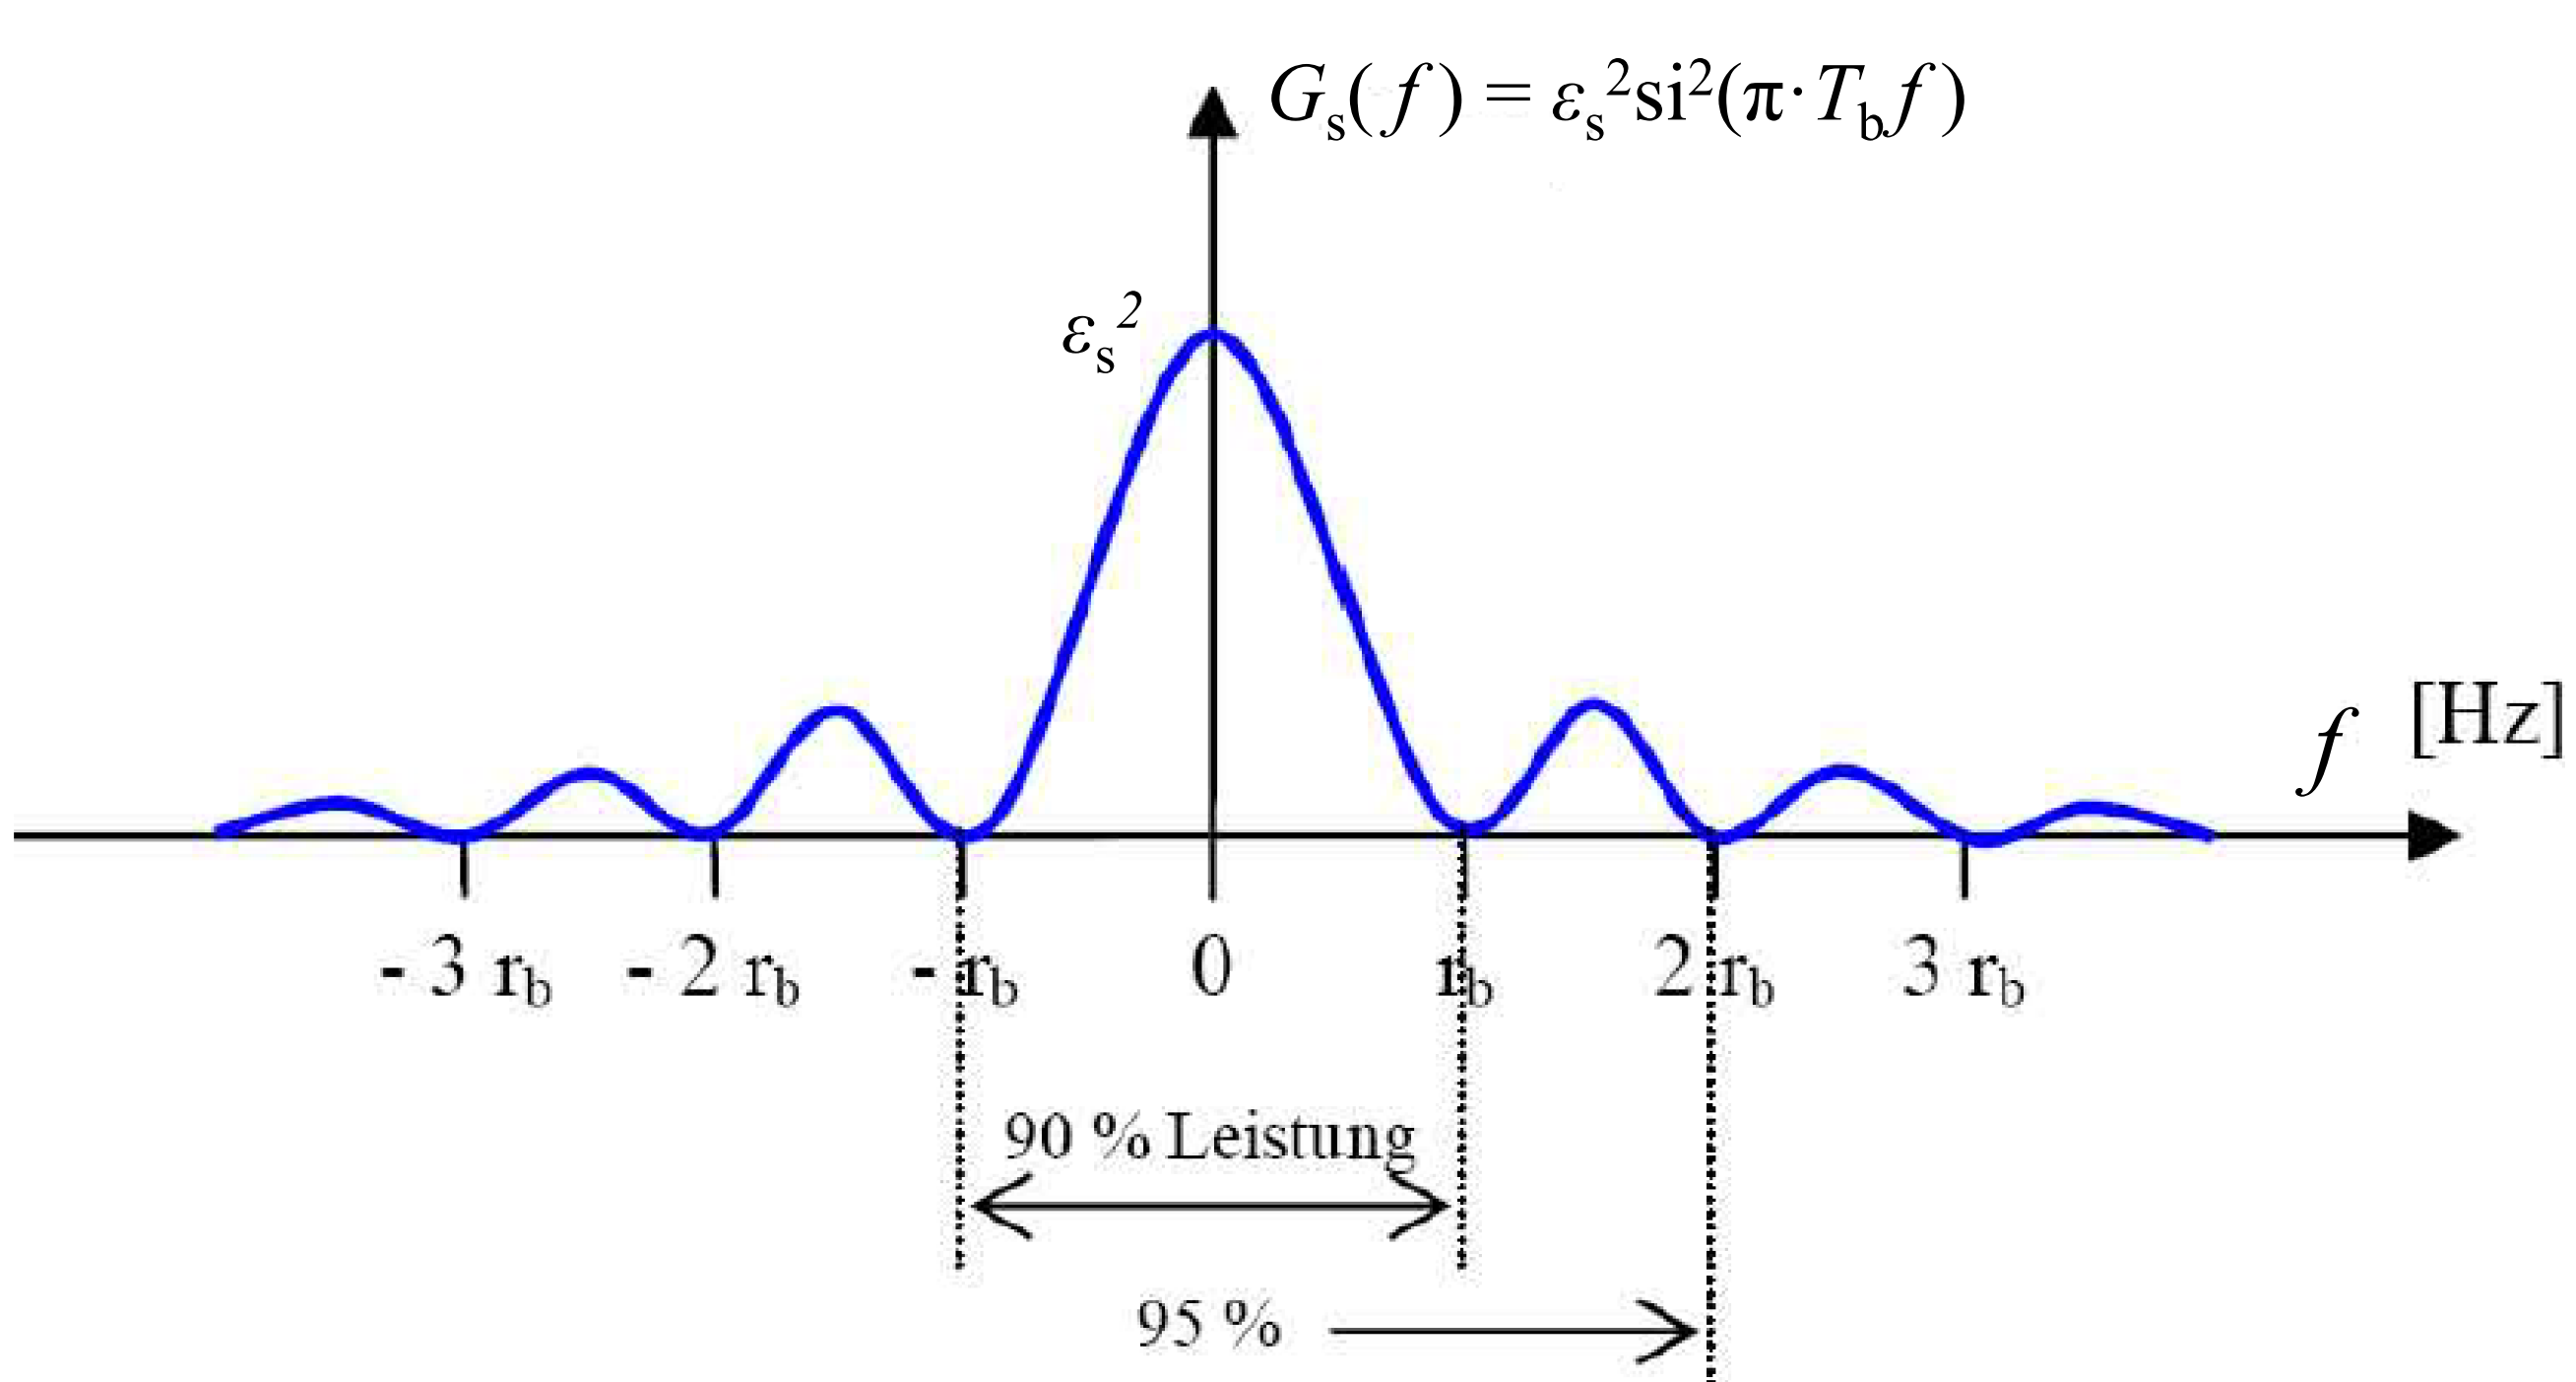
\includegraphics[width=.9\textwidth]{./images/grect}
\end{center}
~\\
si-Impulse:
\[
	p_{si}(t) = T_b^{-\frac{1}{2}} \cdot \textrm{si}(\pi r_b t)
\]
\begin{center}
	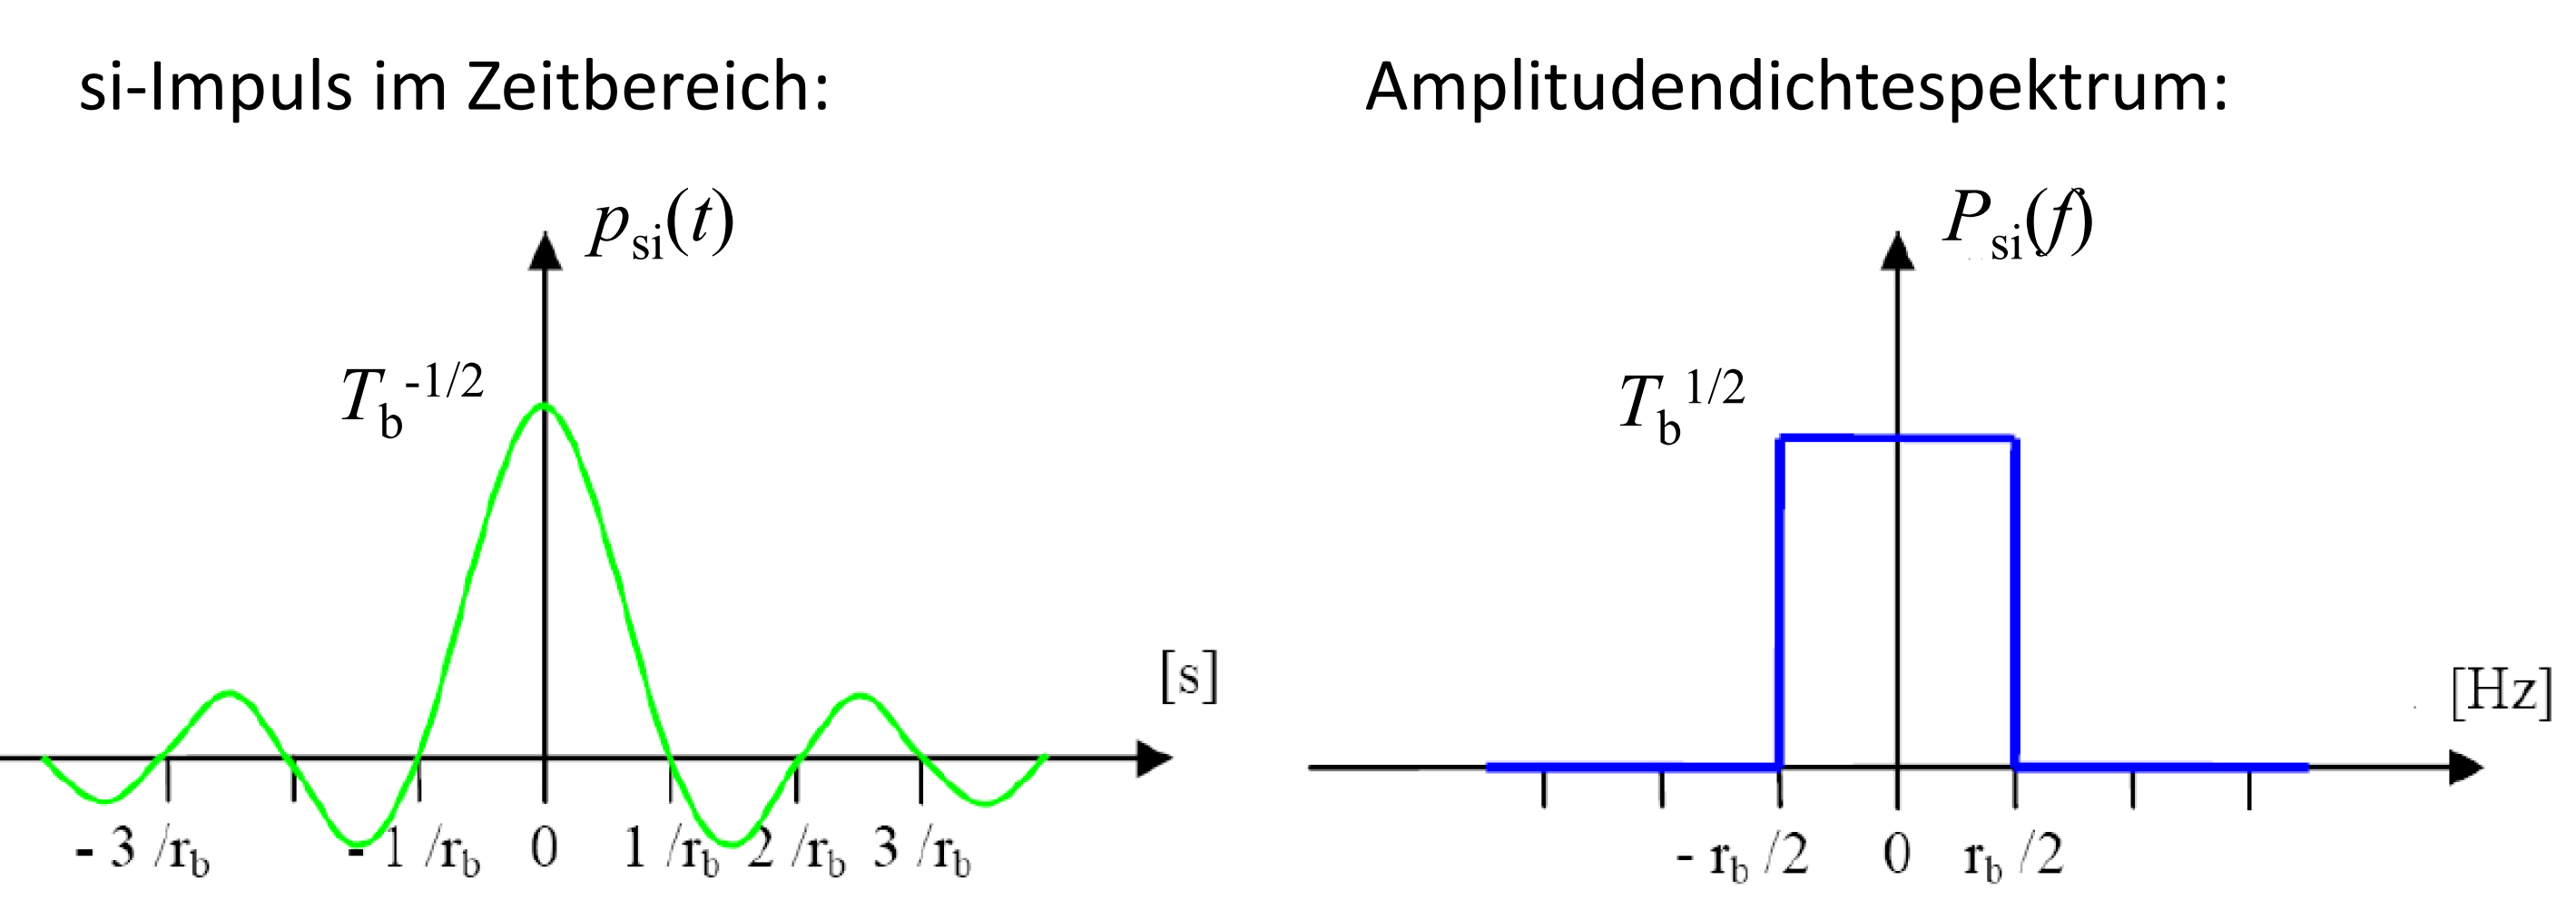
\includegraphics[width=.9\textwidth]{./images/si}
\end{center}

\section{ISI-freie Detektion}
Eine Abtastung zu idealen Zeitpunkten ermöglicht eine ISI-freie Detetkion wenn:
\[\begin{aligned}
	p(0) &= A\\
	p(nT_b) &= 0 \qquad \textrm{, für } n=\pm1,\pm2,\ldots	
\end{aligned}\]
~\\Gemäss Nyquist erfüllt wenn:
\[
	\sum_{k=-\infty}^{\infty} P\left(f+\frac{k}{T_b}\right) = AT_b
\]

\section{raised-Cosine-Spectrum}
\[
	P_{rc}(f) = \left\lbrace
	\begin{matrix}
		AT_b & \textrm{, für } 0 \leq |f| \leq \frac{1-\alpha}{2T_b} \\
		\frac{AT_b}{2}\left(1 + \cos\left( \frac{\pi T_b}{\alpha}
			\left(|f|-\frac{1-\alpha}{2T_b} \right)\right)\right)
			& \textrm{, für } \frac{1-\alpha}{2T_b} \leq |f| \leq \frac{1+\alpha}{2T_b} \\
			0 & \textrm{, für } |f| > \frac{1+\alpha}{2T_b}
	\end{matrix}
	\right.
\]

\begin{center}
	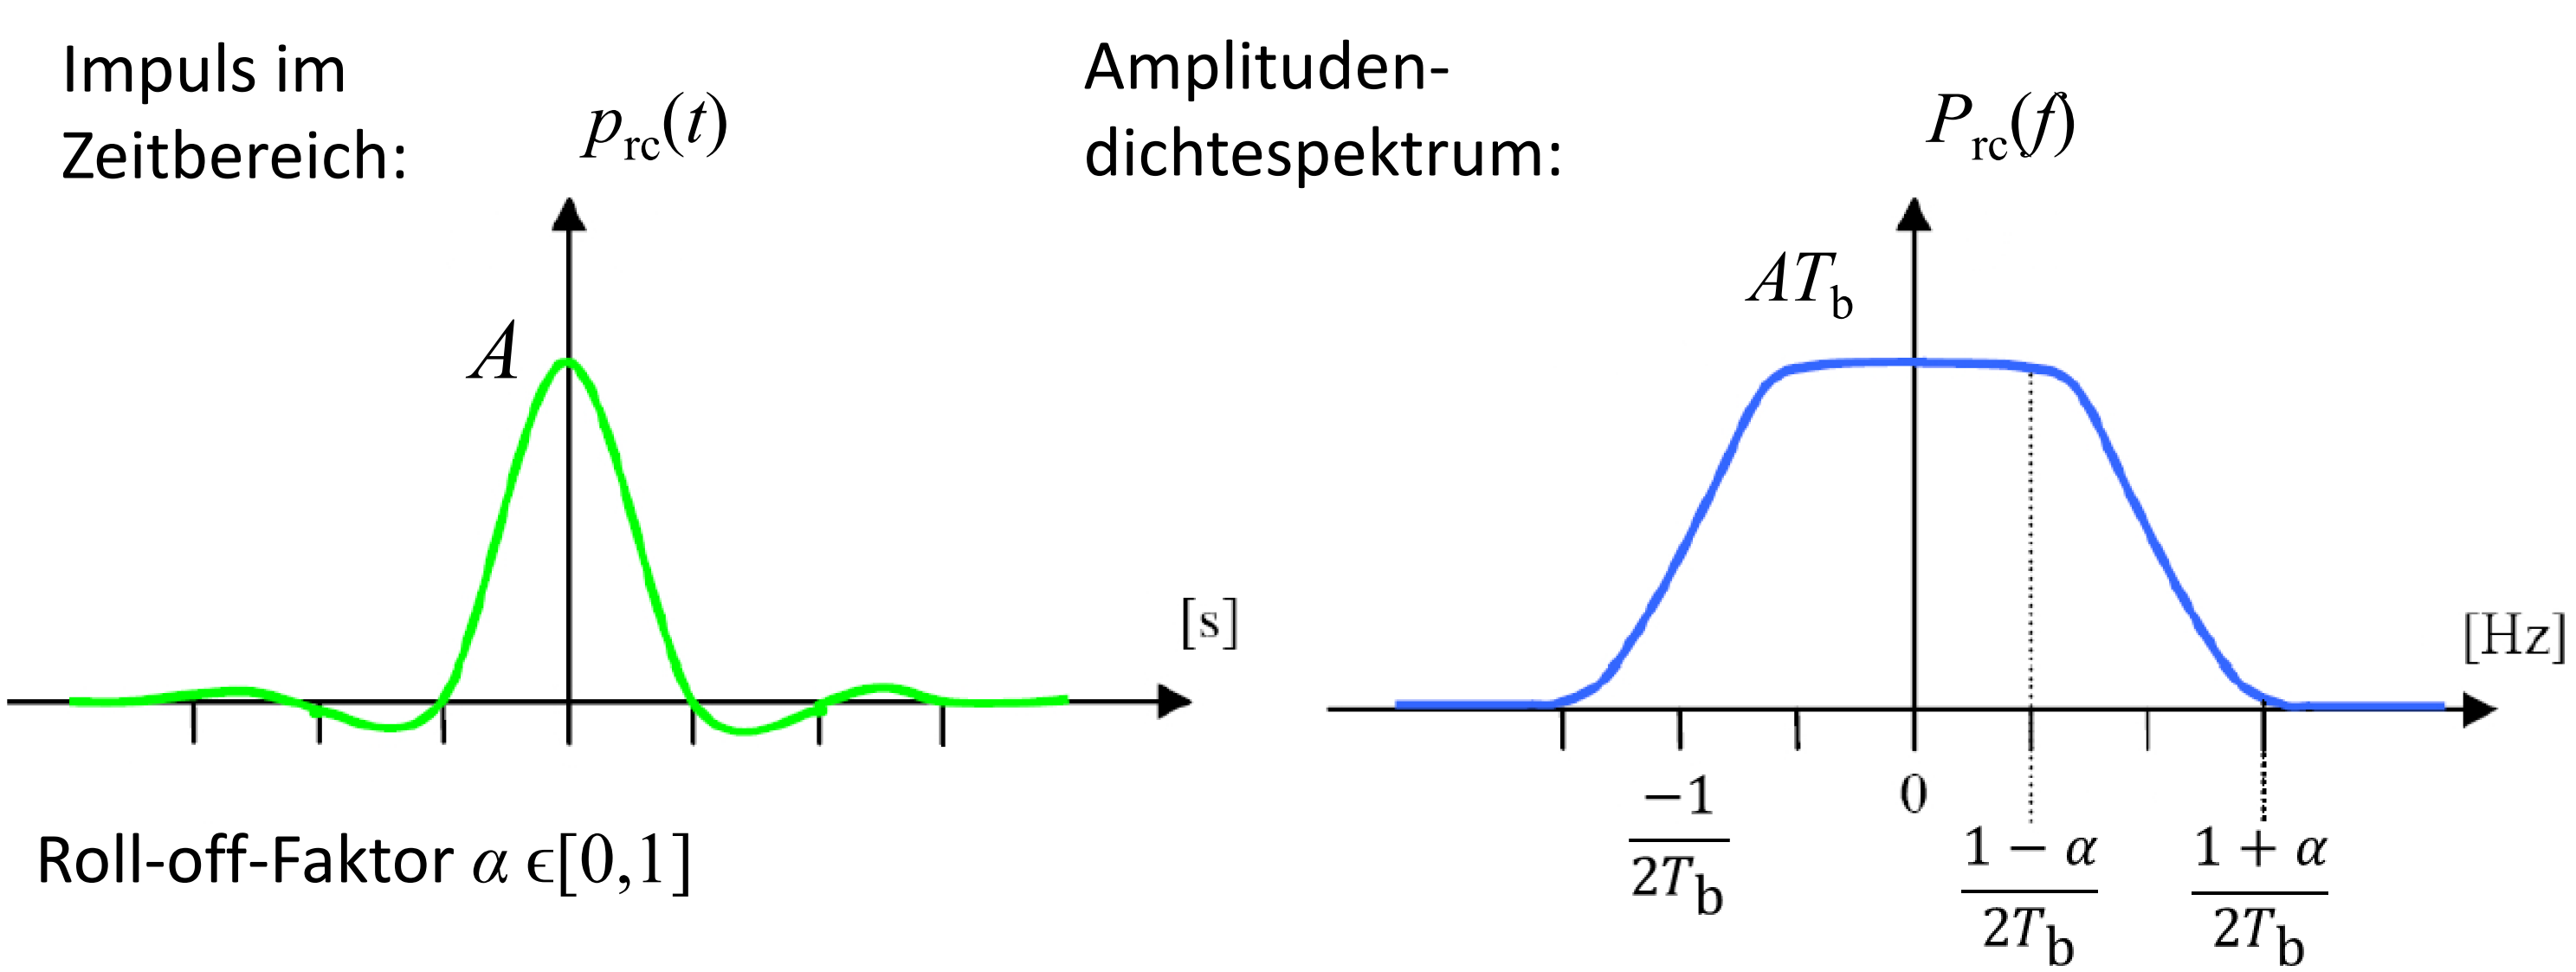
\includegraphics[width=.9\textwidth]{./images/raisedcos.png}
\end{center}

\begin{center}
	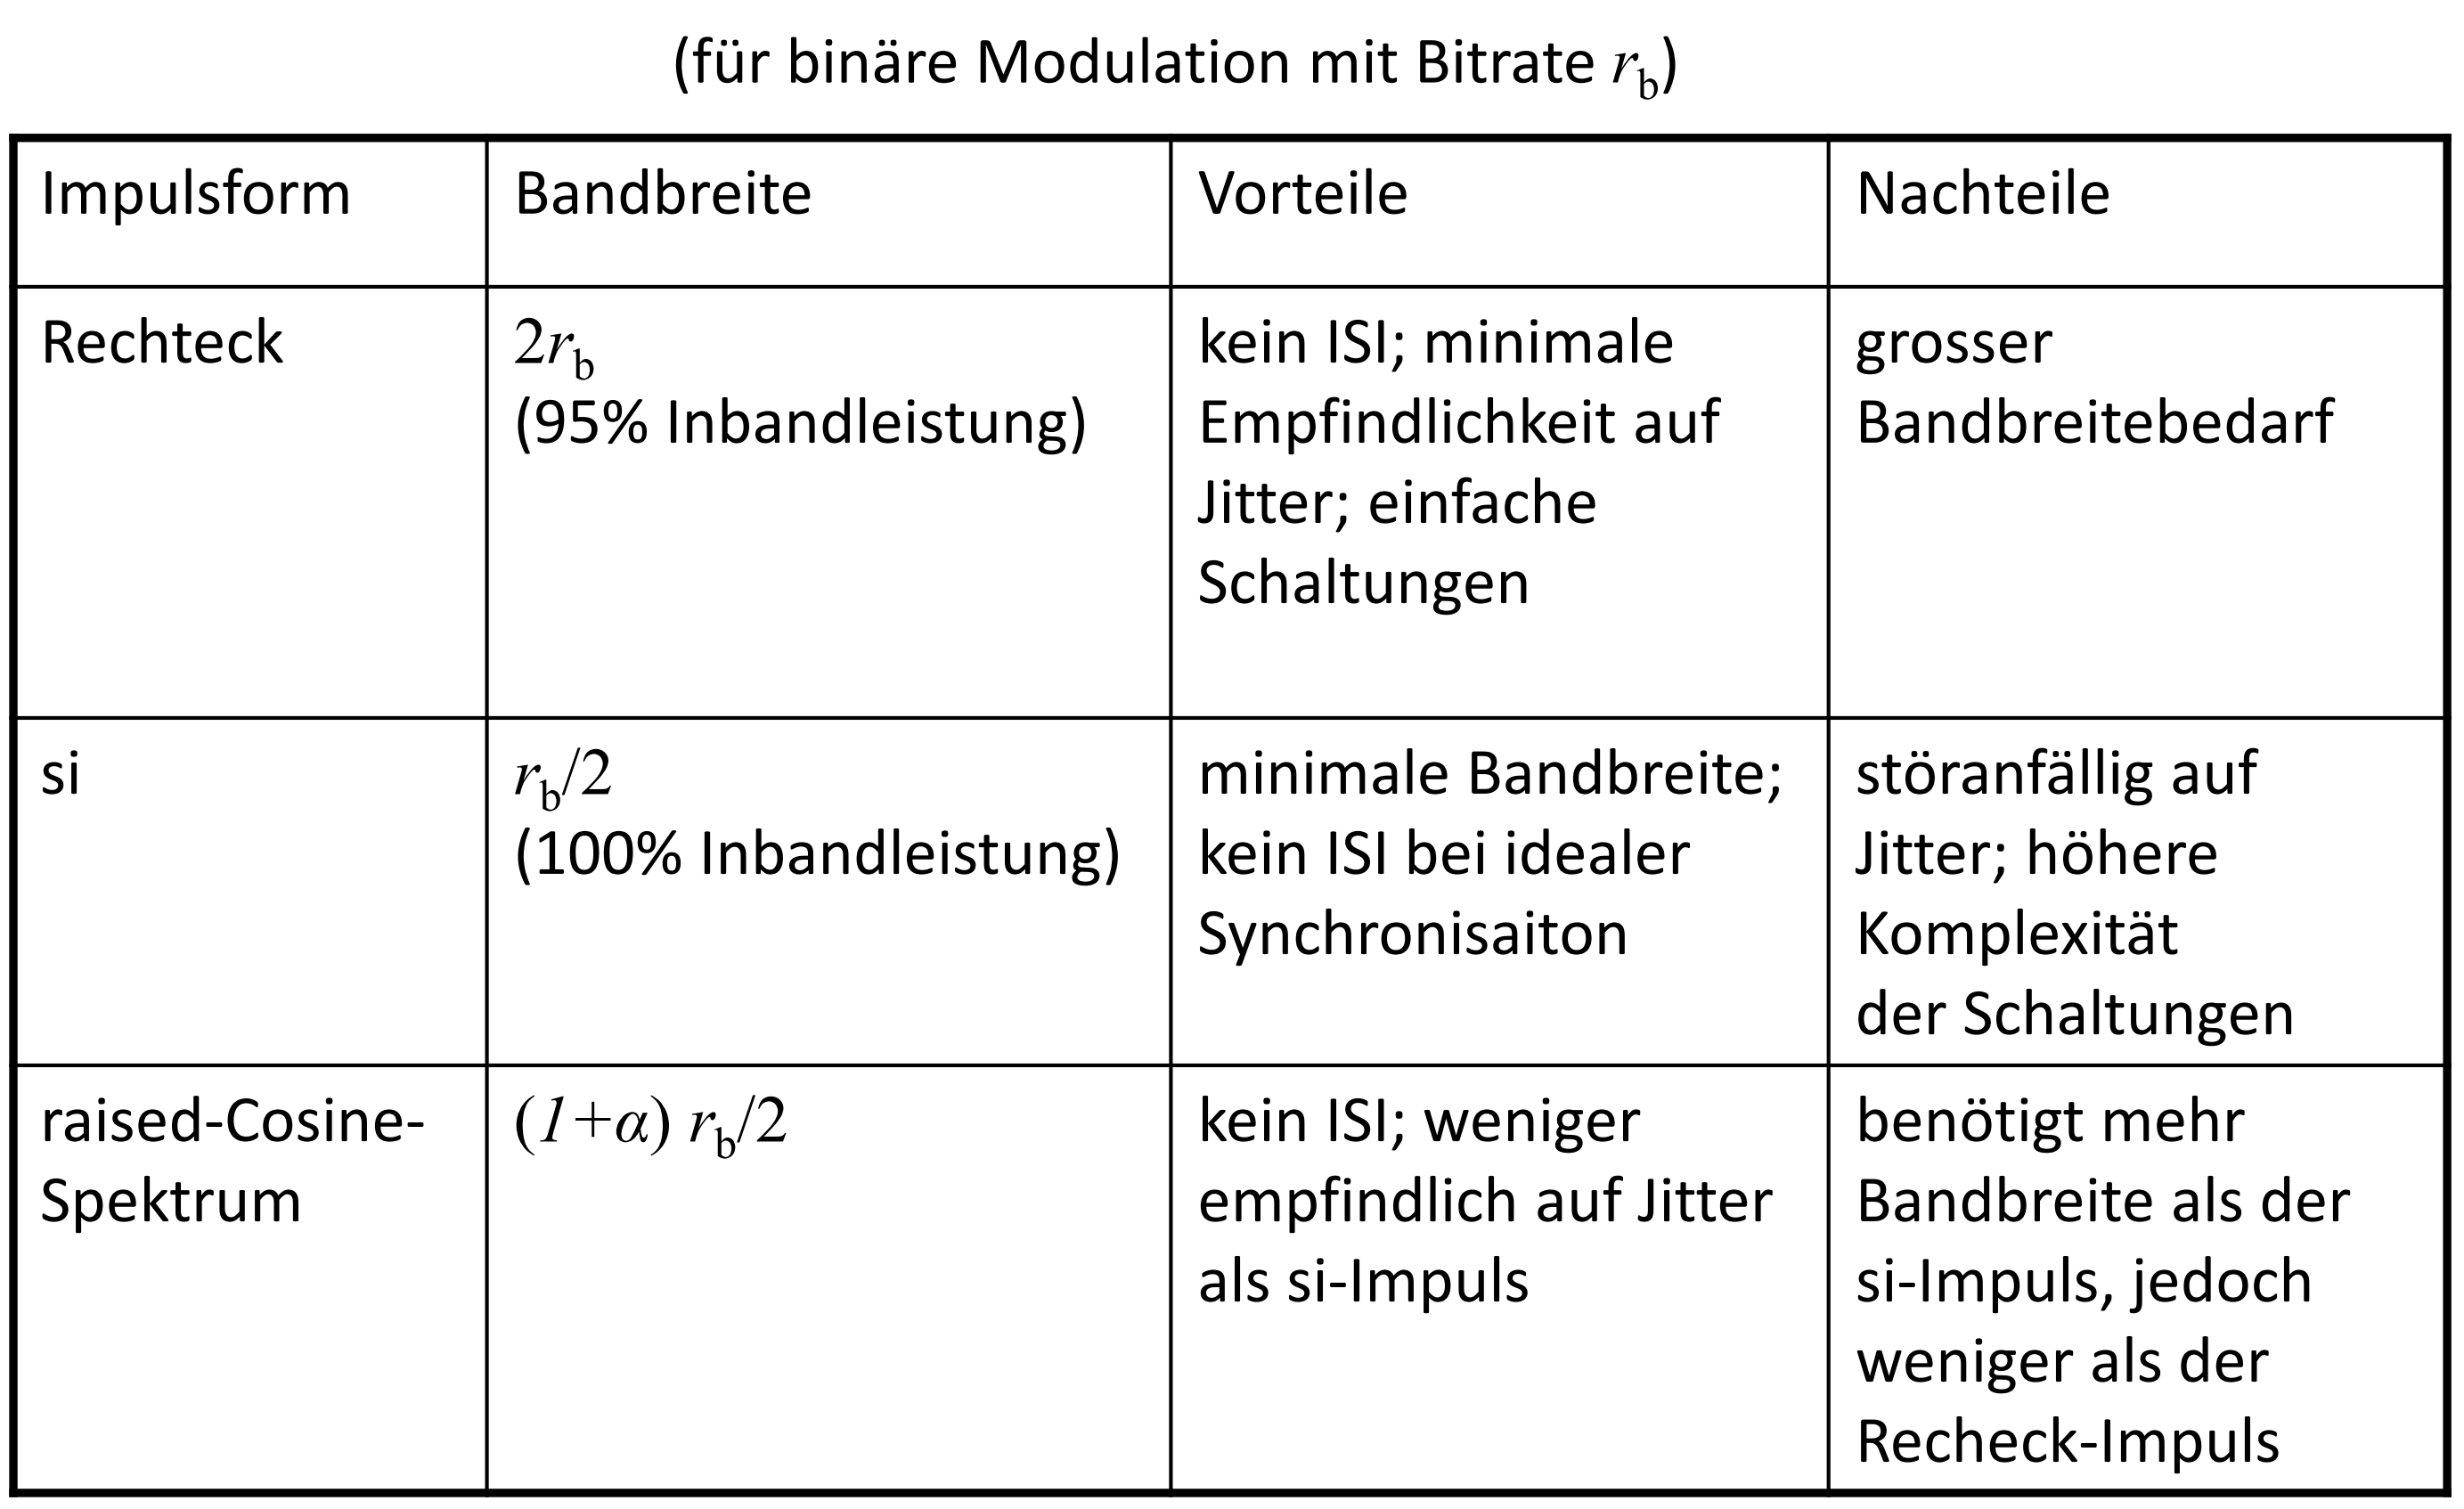
\includegraphics[width=.9\textwidth]{./images/vergleich.png}
\end{center}